\section{Working in Kubernetes}

\subsection{Objectives}
	\begin{frame}
		\frametitle{Objectives}
		Now that we have a worker, we want to run it in a kubernetes cluster.
		
		\bigskip
		The first step will be to run a container into kubernetes to make sure that we can do it.
		
		\bigskip
		Then, we will run our worker in kubernetes.	
	\end{frame}
	
	\begin{frame}[fragile]
		\frametitle{Using minikube}
	
		For the following, make sure that minikube is started:
		\begin{block}{Command terminal}
			\begin{verbatim}
				minikube start
			\end{verbatim}
		\end{block}
	
		Check minikube status:
		\begin{block}{Command terminal}
			\begin{verbatim}
				minikube status
			\end{verbatim}
		\end{block}
	\end{frame}
	
\subsection{Configuring the environment}
	
	\begin{frame}
		\frametitle{Accessing a Kubernetes cluster}
		
		To access a kubernetes cluster, we use kubectl client configured with the file \textit{ \$home/.kube/config}
		
		More information \href{https://kubernetes.io/docs/tasks/access-application-cluster/configure-access-multiple-clusters/}{here}.
		
		\bigskip
		
		As we are using Minikube, starting it already configures kubectl.
		
		\bigskip
		
		As indicated in \href{https://kubernetes.io/docs/tasks/tools/install-kubectl/\#enabling-shell-autocompletion}{this documentation}, you can enable the completion for kubectl.
		
	\end{frame}
	
\subsection{Running a container in kubernetes}	
		
	\begin{frame}[fragile]
		\frametitle{Running our first container in the cluster}
	
		To begin, we are just going to deploy a container sending a ping:
		\begin{block}{Command terminal}
			\begin{verbatim}
				kubectl run pingpong --image=alpine ping 1.1.1.1
				
				kubectl get deployments -o wide
				kubectl get replicaset -o wide
				kubectl get pods -o wide
			\end{verbatim}
		\end{block}
	\end{frame}
	
	\begin{frame}
		\frametitle{Kubernetes application architecture}
		
		\begin{center}
		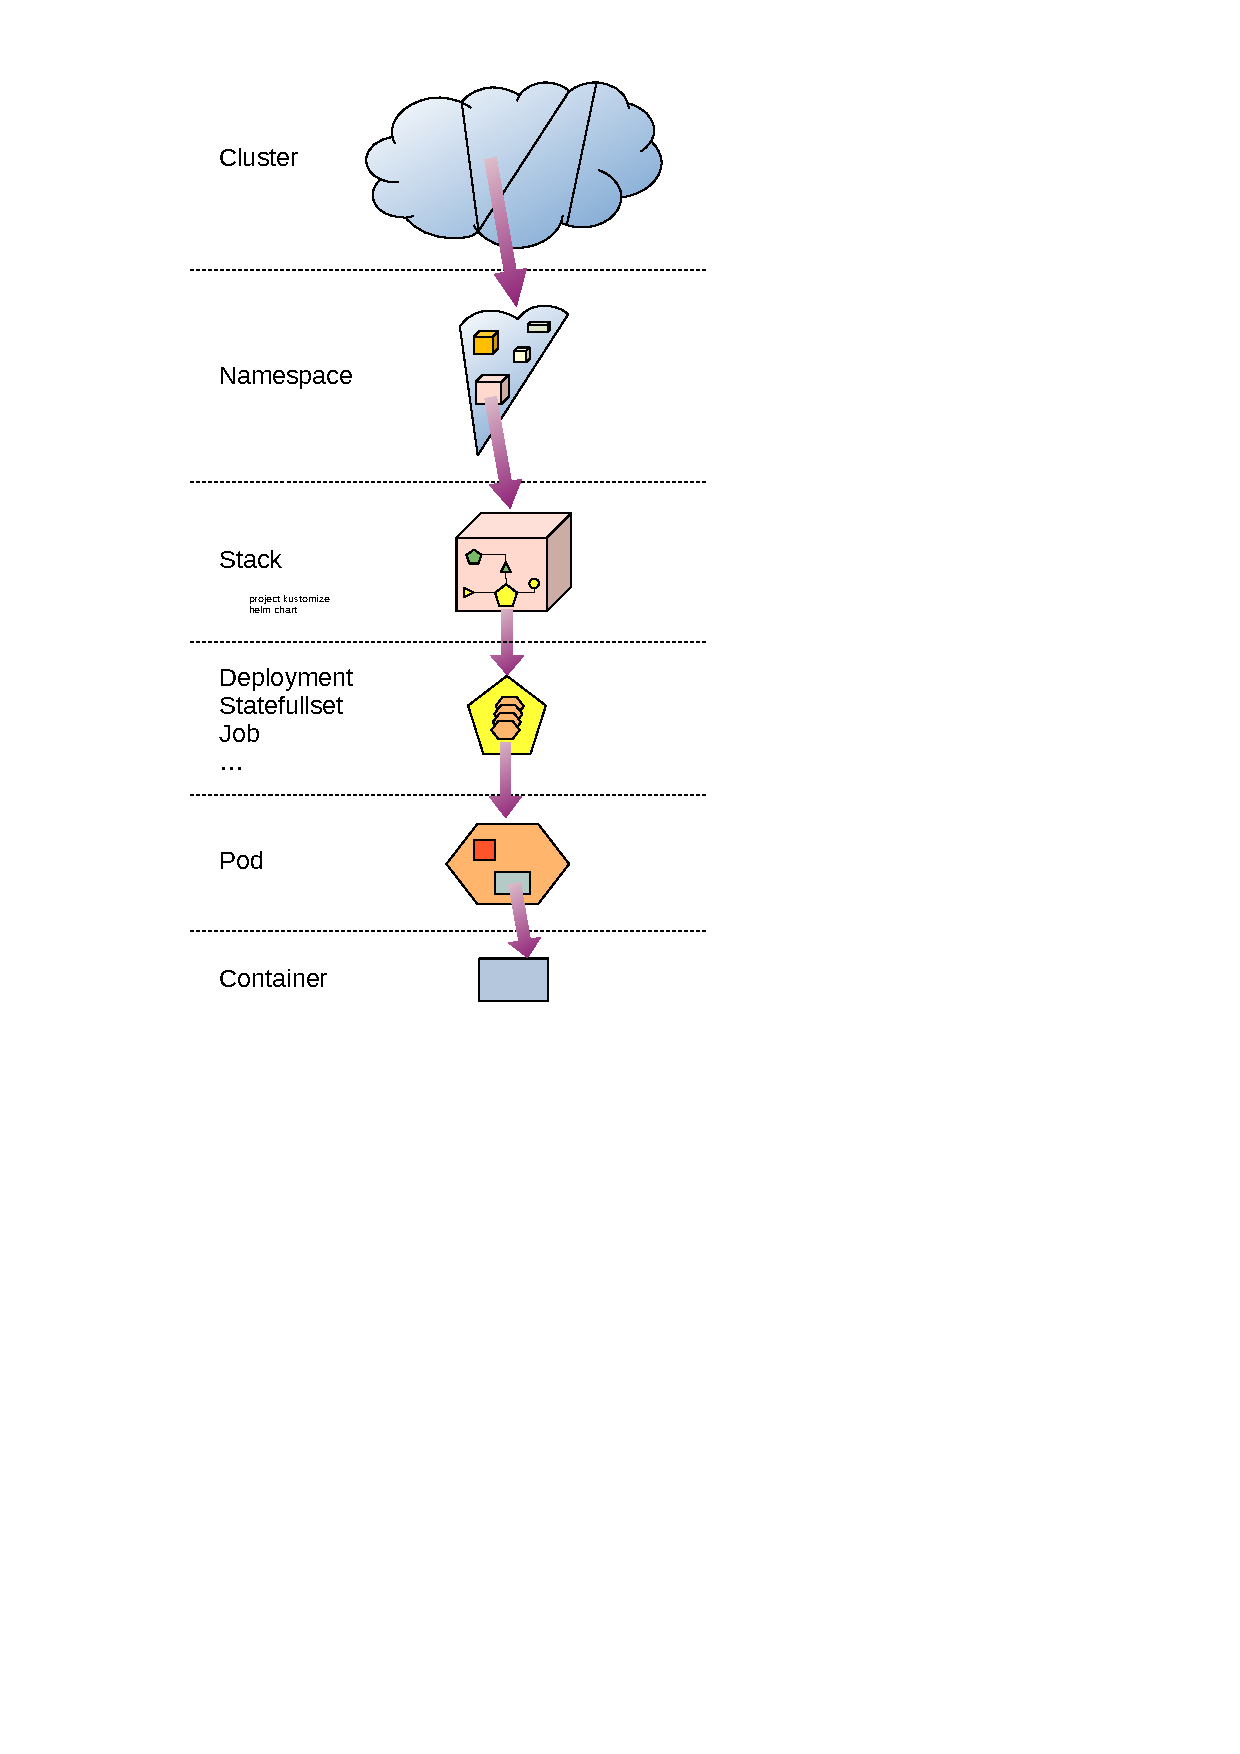
\includegraphics[height=7cm]{../../../resources/color/fromCluster2container.pdf}
		\end{center}
		
	\end{frame}		

	\begin{frame}
		\frametitle{Preparing the environment}
		
		Starting from now, we are going to use 3 shells in 3 differents windows/panes.
		
	\end{frame}		

	\begin{frame}[fragile]
		\frametitle{Looking at logs in a kubernetes cluster}
	
		We want to display the logs of this container:
		\begin{block}{Logs terminal}
			\begin{verbatim}
				kubectl logs -f pingpong-XXXX-XXXX
			\end{verbatim}
		\end{block}
		
		Something happens and we need to recreate the pod:
		\begin{block}{Monitor terminal}
			\begin{verbatim}
				kubectl get pods -w
			\end{verbatim}
		\end{block}
		\begin{block}{Commands terminal}
			\begin{verbatim}
				kubectl delete pod pingpong-XXXX-XXXX
			\end{verbatim}
		\end{block}
	\end{frame}
	
% Use the pods start section to explain kubernetes internal behavior and stress the difference between kubectl API OK response and effective command execution	
	
	\begin{frame}[fragile]
		\frametitle{Looking at logs in a kubernetes cluster}
	
		There are several problems:
		\begin{itemize}
			\item[$\bullet$] we do not see which logs comes from which pod
			\item[$\bullet$] in fact we do not see the new containers logs
		\end{itemize}

		\medskip		
		
		How to solve this and be able to follow logs even if pods are moving?
	\end{frame}

	\begin{frame}[fragile]
		\frametitle{Using stern to look at logs}

		So, we are going to redo the operation but this time using stern:
		\begin{block}{Command terminal}
			\begin{verbatim}
				stern pingpong
			\end{verbatim}
		\end{block}
				\begin{block}{Monitor terminal}
			\begin{verbatim}
				watch kubectl get all
			\end{verbatim}
		\end{block}
		\begin{block}{Second command terminal}
			\begin{verbatim}
				kubectl delete pod pingpong-XXXX-XXXX
			\end{verbatim}
		\end{block}
	\end{frame}
	
	\begin{frame}[fragile]
		\frametitle{Cleaning up the namespace}
		
		Before returning to our worker, a little cleaning can be wise:
		\begin{block}{Command terminal}
			\begin{verbatim}
				kubectl delete deployment pingpong
				kubectl get all
			\end{verbatim}
		\end{block}
		
		\medskip
		
		And stop the commands in the other windows.
	\end{frame}
	
\subsection{Running our worker in kubernetes}

	\begin{frame}[fragile]
		\frametitle{Running our worker in kubernetes}
		
		Now that we know how to run something in kubernetes, we are going to do it with our worker:
		\begin{block}{Logs terminal}
			\begin{verbatim}
				stern worker
			\end{verbatim}
		\end{block}		
		\begin{block}{Monitor terminal}
			\begin{verbatim}
				kubectl get pods -w
			\end{verbatim}
		\end{block}
		\begin{block}{Command terminal}
			\begin{verbatim}
				docker images
				kubectl run worker --image=tinkou/worker:v1
			\end{verbatim}
		\end{block}
	\end{frame}
	
	\begin{frame}[fragile]
		\frametitle{Troubleshooting}
		
		Kubectl get pods indicate that something went wrong.
		
		Check kubernetes object to find the problem root cause:
		\begin{block}{Command terminal}
			\begin{verbatim}
				kubectl	describe deployment worker
				kubectl describe replicaset worker-XXXX
				kubectl describe pod worker-XXXX-XXXX
			\end{verbatim}
		\end{block}
		
		The "Events" are the interesting part here.
		
	\end{frame}
	
	\begin{frame}[fragile]
		\frametitle{Using a registry}
		
		The events indicates that the image can not be found.
		
		\medskip
		
		The docker daemon in minikube is not the same as the local one.
		
		\medskip 
		We need to:
		\begin{itemize}
			\item link the local docker CLI to the minikube docker daemon
			\item create the image in the minikube docker daemon locale registry
		\end{itemize}
		
		\begin{block}{Command terminal}
			\begin{verbatim}
				eval $(minikube docker-env)
				docker images
				docker build -t tinkou/worker:v1 .
			\end{verbatim}
		\end{block}

	\end{frame}
	
	\begin{frame}[fragile]
		\frametitle{Using a registry}
	
		After a moment, the pod and stern starts displaying logs. What happened?
		
		\bigskip
		
		\visible<2->{
			The different elements of kubernetes retry periodically. And as the image is now available, the pods can successfully start.
		}
	
	\end{frame}


	\begin{frame}
		\begin{center}
			Questions?
		\end{center}
	\end{frame}